\section{Results}
\label{sec:results}
Every number below is read from \texttt{results/} by \texttt{experiments/e7\_numbers.py}.

\subsection{Certified DC robust secure set (E1)}
All \NEbProblems\ bilevel problems (24 hours, upper and lower limit) were solved to
certified optimality (master bound equals the attained value to $10^{-9}$). In
\NBendersOneIter\ of them the robust value-function cut is tight and Benders stops after
one master solve; one problem (hour 21, upper) needed phase~2. Mean time is
\NBendersMeanS\,s against \NMilpMeanS\,s for the big-M MILP of the dissertation code
(both with HiGHS on the same CPU), but the more important difference is correctness
(Fig.~\ref{fig:dc}b): the MILP's reported objective differs from the value its own
leader decision attains in \NBigmErrN\ of \NEbProblems\ problems, by up to
\NBigmErrMaxMw\,MW (hour \NBigmErrHour, \NBigmErrLimit\ limit), and in
\NBigmSuboptN\ problem its leader decision is not optimal. This is the known failure
mode of a fixed big-M in bilevel KKT reformulations~\cite{pineda2019bigm}; the Benders
certificate removes it. The mean DC secure range is \NDcWidthMeanMw\,MW.

\begin{figure*}[t]
\centering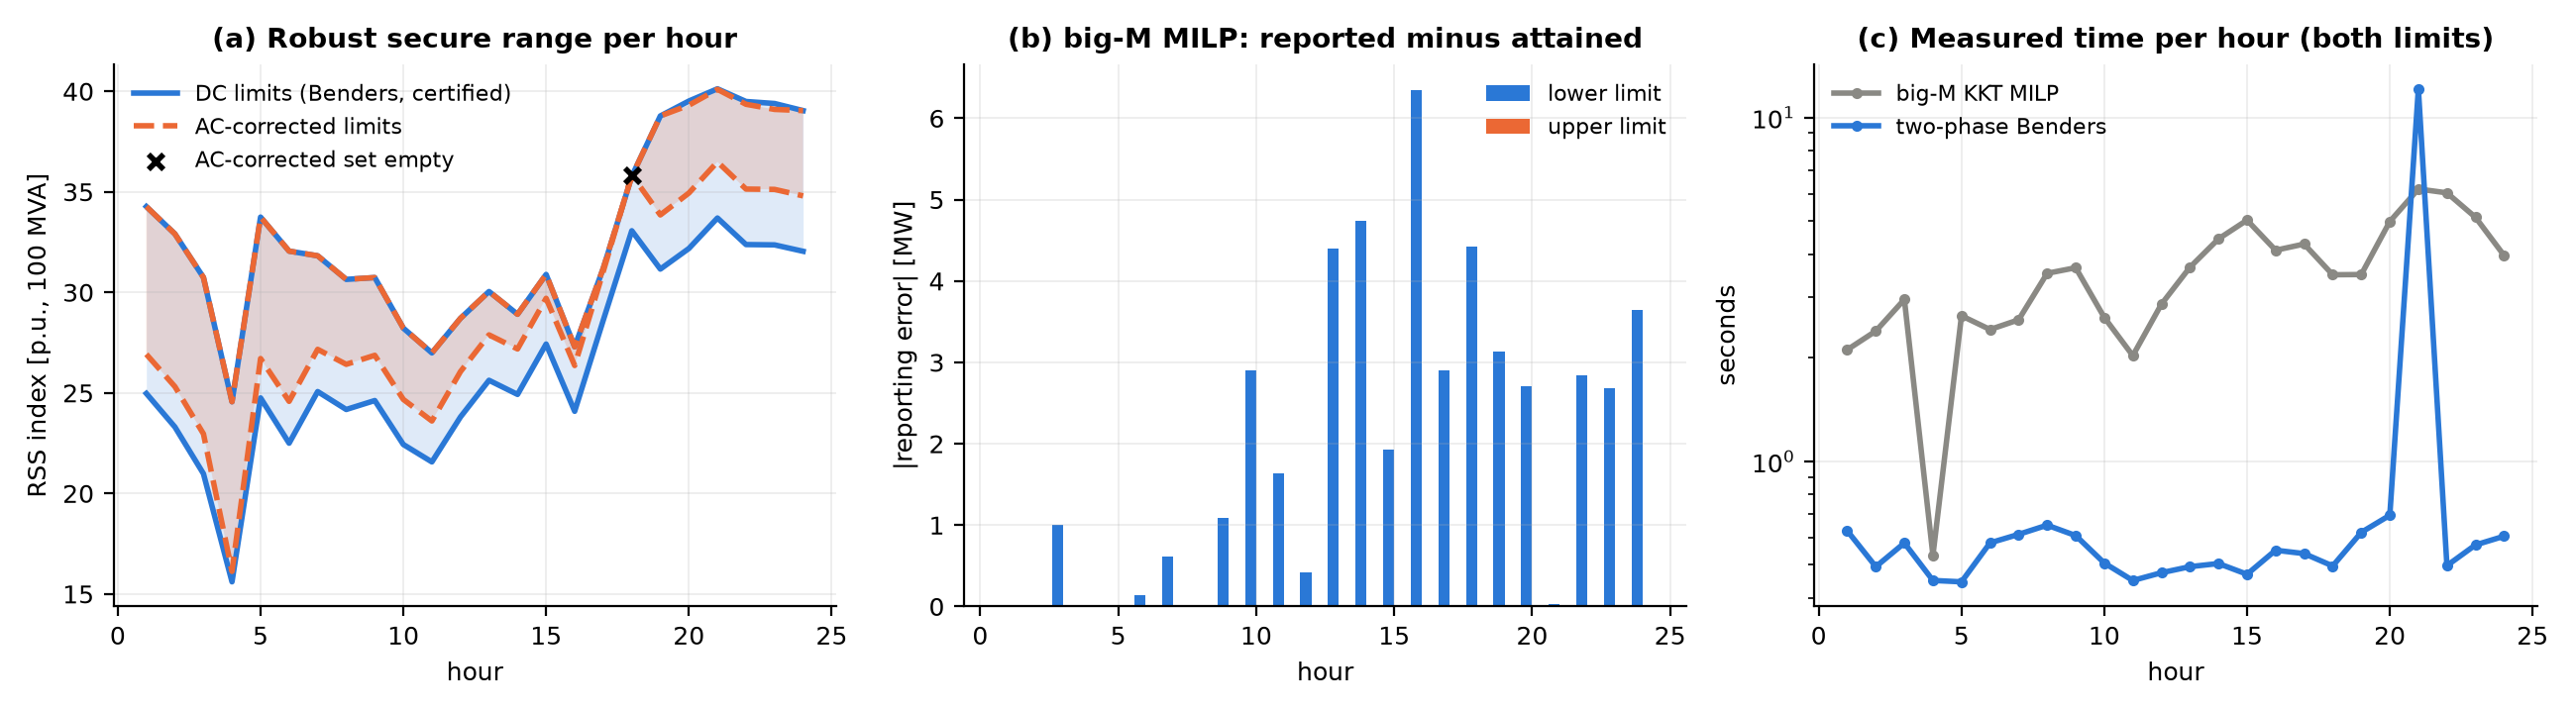
\includegraphics[width=\textwidth]{../results/figures/fig1_dc_rss.png}
\caption{(a) Certified DC limits per hour and AC-corrected limits from the GENCO-in-the-loop
correction (E4). (b) Big-M MILP: reported objective minus value attained by its leader
decision. (c) Measured solve time.}
\label{fig:dc}
\end{figure*}

\subsection{GENCO accuracy and its corrective-layer trajectory (E3)}
The trained GENCO (\NGencoParams\ parameters) predicts the maximum branch loading
with mean absolute error \NLoadMaeIidPct\,\% (training distribution),
\NLoadMaeScreenPct\,\% (screening distribution) and \NLoadMaeUnseenPct\,\% (unseen
topology) of the rating, and
voltage magnitudes with mean worst-bus error \NVmErrScreen\,p.u. The error is
\emph{not} uniform (Fig.~\ref{fig:probe}a): GENCO under-predicts a cluster of
contingency-100--103 scenarios. Inside GENCO the AC mismatch contracts by more than two
orders of magnitude over the $K=10$ layers, and almost identically in the unseen
topology (Fig.~\ref{fig:probe}b). Single scalars of that trajectory are weak error
indicators (Spearman \NSpRlast\ for $\bar r^{(K)}$, AUROC \NAucRlast\ for the 10\,\%
largest errors, \NOodAucRlast\ for detecting the unseen topology). The \emph{whole}
trajectory is informative (Fig.~\ref{fig:probe}c): a recalibrator that sees only
$\bar r^{(1)},\dots,\bar r^{(K)},\rho$ removes \NTrajOnlyMaeRedPct\,\% of the error, and PTR
(trajectory plus GENCO outputs) removes \NPtrMaeRedPct\,\% (MAE \NRawMaeTestPct\,\%
$\to$ \NPtrMaeTestPct\,\%) and reduces it in the unseen topology from
\NRawMaeUnseenPct\,\% to \NPtrMaeUnseenPct\,\%.

\begin{figure*}[t]
\centering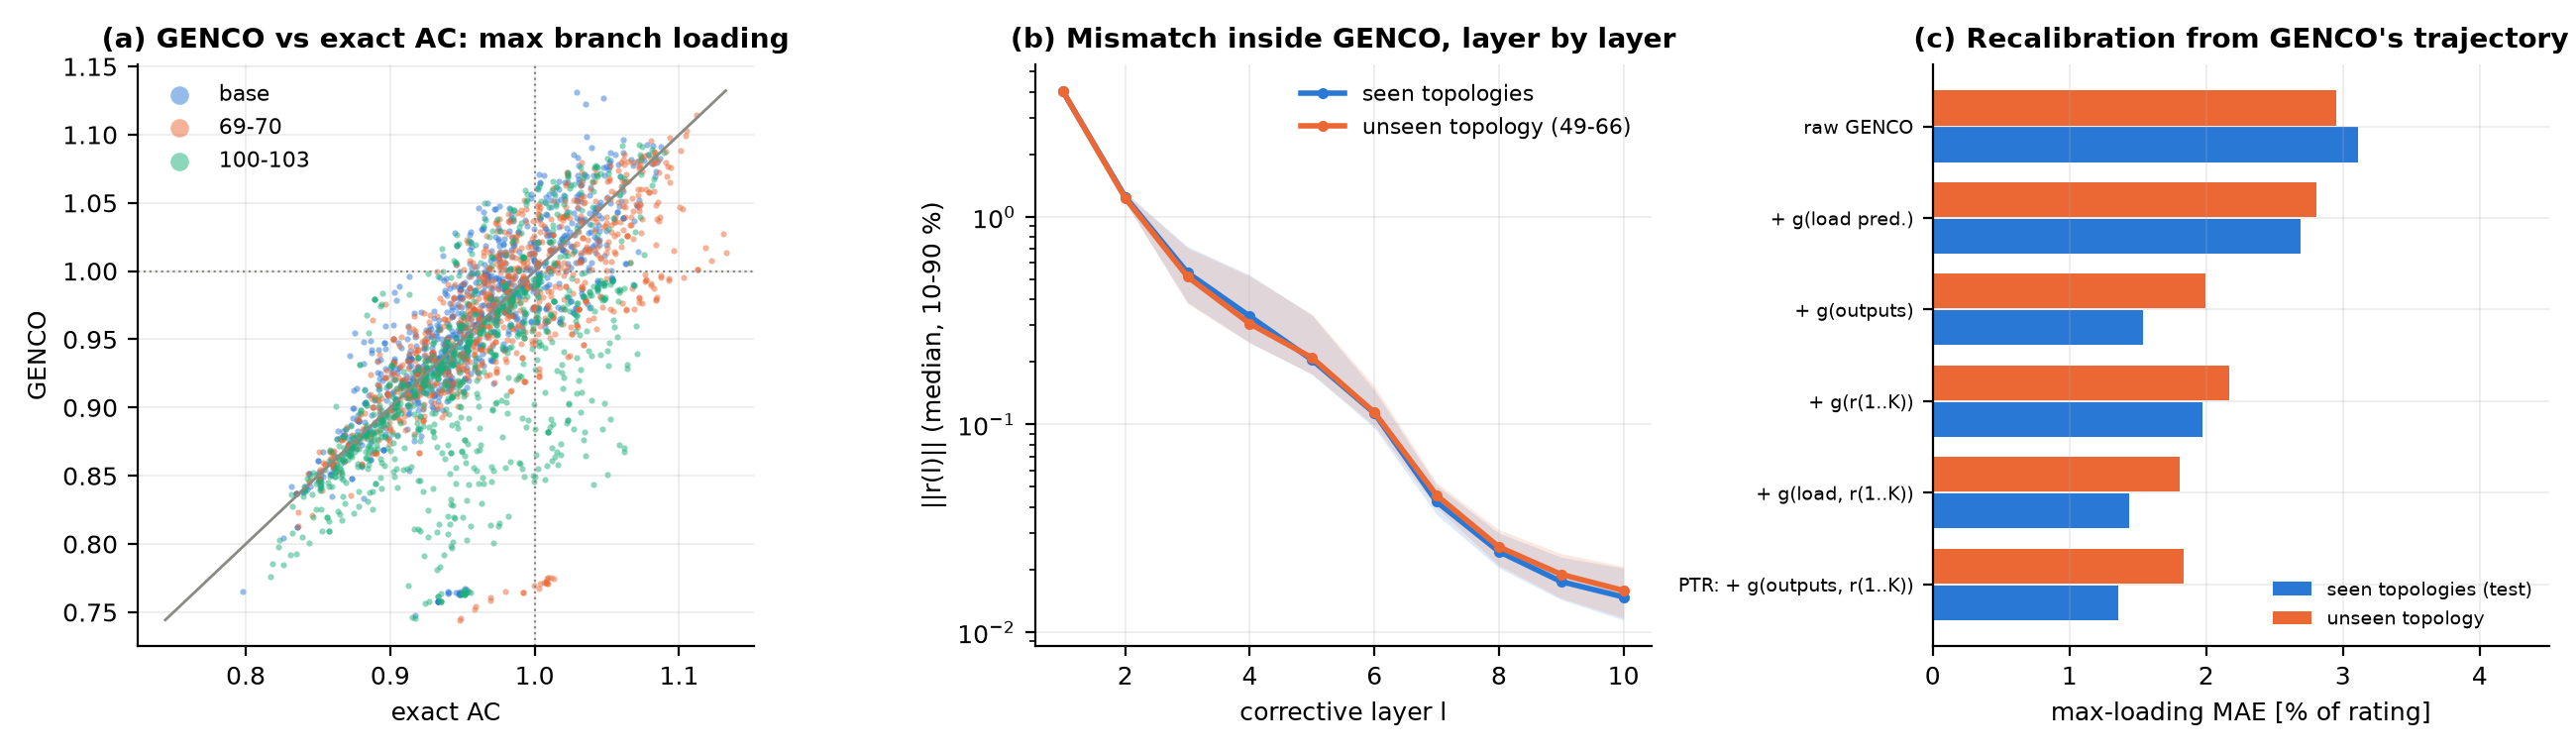
\includegraphics[width=\textwidth]{../results/figures/fig2_genco_probe.png}
\caption{(a) GENCO vs.\ exact AC (screening test set), by topology. (b) AC mismatch
measured inside GENCO, layer by layer. (c) Ablation: what the recalibrator sees vs.\
remaining error (fitted on the tune split, evaluated on test and unseen topology).}
\label{fig:probe}
\end{figure*}

\subsection{Screening with a guarantee (E3)}
Table~\ref{tab:conf} and Fig.~\ref{fig:conf} report the screening over \NNSplits\ random
tune/calibration/test splits of the 3{,}000 screening scenarios (\NTestInsecure\ of
\NTestN\ test scenarios are insecure: the screening distribution sits on the RSS
boundary by construction). At $\alpha=0.05$, plain split-conformal screening can clear
only \NClearPlainAaf\,\% of the secure scenarios, because GENCO's error tail forces a wide
margin; PTR clears \NClearPtrAaf\,\% in seen topologies and \NClearUnseenPtrAaf\,\% in
the unseen one. The observed rate of insecure-and-cleared scenarios is
\NMissPtrAaf\,\% (worst split \NMissmaxPtrAaf\,\%), far below the 5\,\% guarantee.

\begin{table}[t]
\centering
\caption{Secure scenarios cleared without exact AC [\%] and observed miss rate [\%]
(mean of \NNSplits\ splits; miss = insecure and cleared).}
\label{tab:conf}
\setlength{\tabcolsep}{3.5pt}
\begin{tabular}{@{}llccc@{}}
\toprule
 & & $\alpha=0.01$ & $\alpha=0.05$ & $\alpha=0.10$\\
\midrule
\multirow{3}{*}{\shortstack[l]{seen\\topol.}}
 & plain      & \NClearPlainAab & \NClearPlainAaf & \NClearPlainAb\\
 & normalised & \NClearNormalisedAab & \NClearNormalisedAaf & \NClearNormalisedAb\\
 & PTR        & \textbf{\NClearPtrAab} & \textbf{\NClearPtrAaf} & \textbf{\NClearPtrAb}\\
 & PTR miss   & \NMissPtrAab & \NMissPtrAaf & \NMissPtrAb\\
\midrule
\multirow{3}{*}{\shortstack[l]{unseen\\49--66}}
 & plain      & \NClearUnseenPlainAab & \NClearUnseenPlainAaf & \NClearUnseenPlainAb\\
 & normalised & \NClearUnseenNormalisedAab & \NClearUnseenNormalisedAaf & \NClearUnseenNormalisedAb\\
 & PTR        & \textbf{\NClearUnseenPtrAab} & \textbf{\NClearUnseenPtrAaf} & \textbf{\NClearUnseenPtrAb}\\
 & PTR miss   & \NMissUnseenPtrAab & \NMissUnseenPtrAaf & \NMissUnseenPtrAb\\
\bottomrule
\end{tabular}
\end{table}

\begin{figure*}[t]
\centering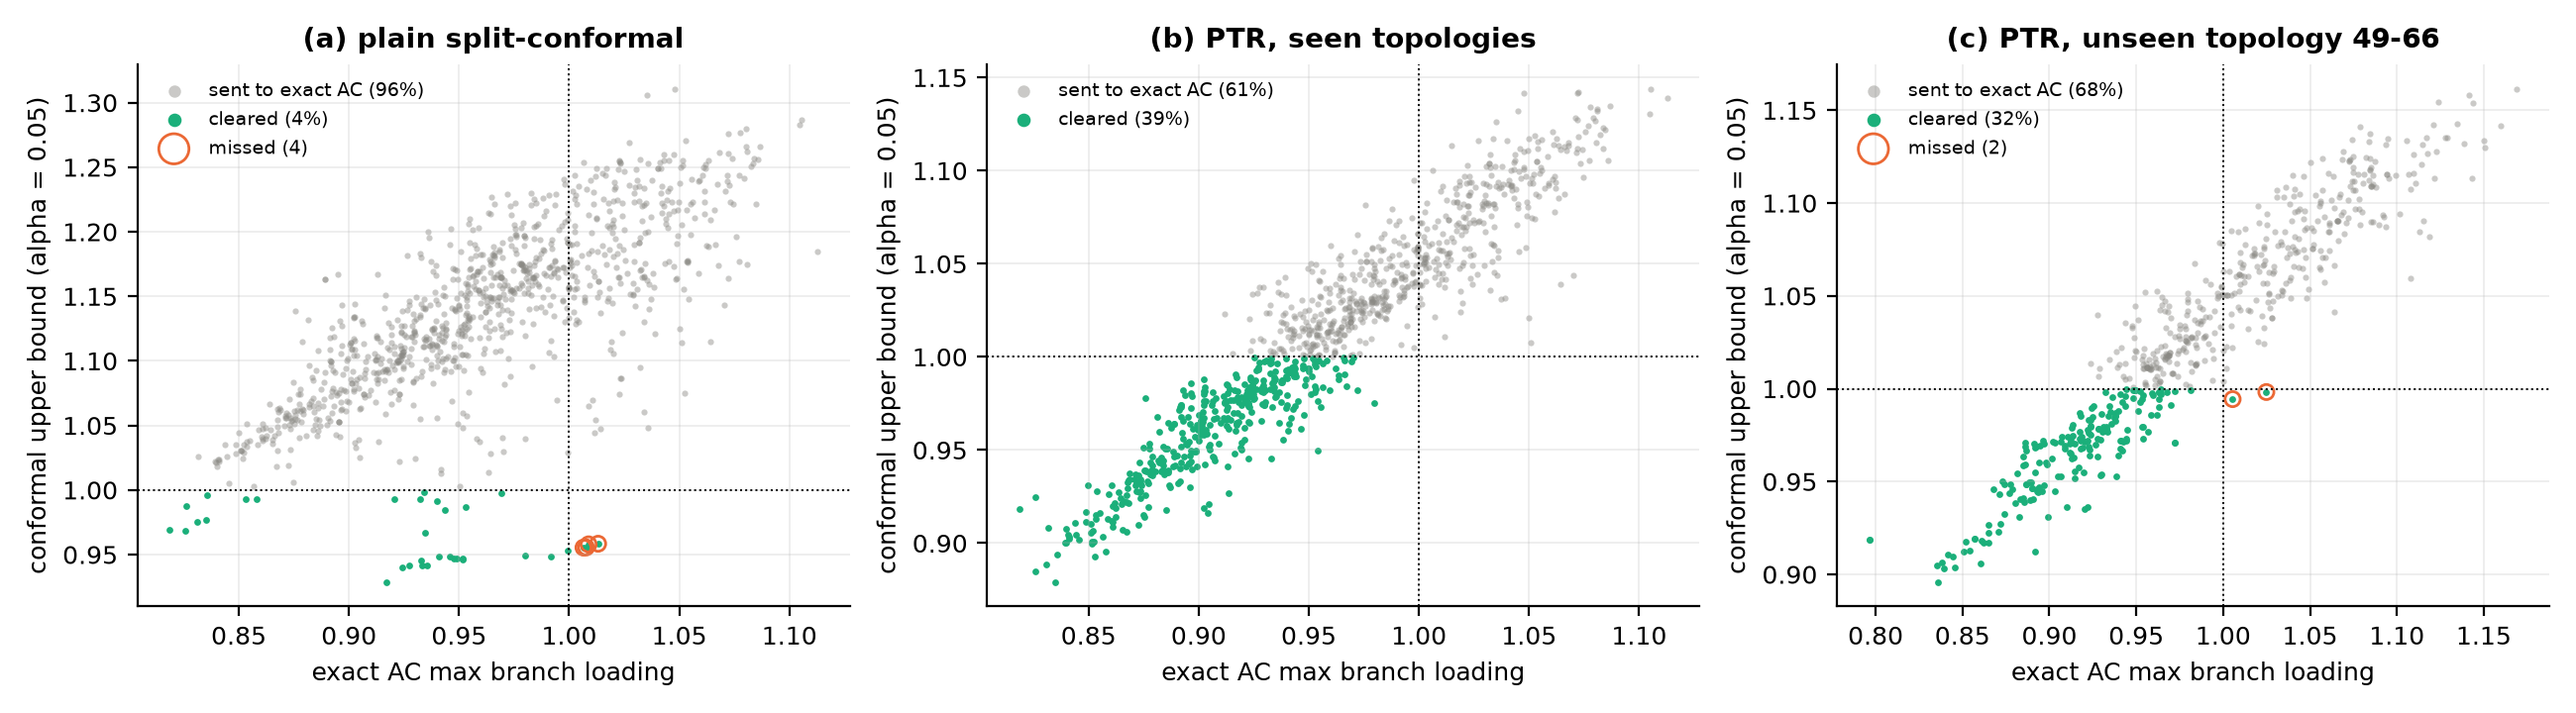
\includegraphics[width=\textwidth]{../results/figures/fig6_screen.png}
\caption{Conformal upper bound on the maximum branch loading vs.\ exact AC at $\alpha=0.05$
(one split). Green: cleared without exact AC. Plain conformal must place almost all
scenarios above 1; PTR clears most secure ones, also in the unseen topology.}
\label{fig:conf}
\end{figure*}

\subsection{AC-corrected robust secure set (E4)}
In \NItbDcBoundaryInsecure\ of \NItbN\ hour-limit problems the certified DC limit is
\emph{not} AC-secure: some vertex of the PV/load box overloads a branch in AC (worst
loading \NItbMaxLoadPct\,\% of rating). The GENCO-in-the-loop correction removes all verified
violations in at most \NEeItersMax\ iterations (\NEeSecondsMean\,s per limit on
average). It moves \NEeChanged\ of \NEeLimits\ limits, by up to \NEeShiftMaxMw\,MW
(hour \NEeShiftMaxHour, \NEeShiftMaxLimit\ limit), and the mean secure range shrinks from
\NEeWidthDcMeanMw\ to \NEeWidthAcMeanMw\,MW (Fig.~\ref{fig:dc}a, Fig.~\ref{fig:ac}a): DC
overstates the range by \NEeWidthRedMeanPct\,\% on average. In hour \NEeEmptyHourList\
the corrected lower limit exceeds the upper one, i.e.\ the corrected model admits no
robust secure dispatch although DC reports a range of \NEeEmptyDcWidthMw\,MW. Over the whole run, PTR
cleared \NPoolClearedPct\,\% of the \NPoolTotal\ pool scenarios (the pools sit on the
boundary, so this is lower than in E3); an audit that solved every pool scenario exactly
found \NMissedTotal\ insecure scenario among the cleared ones (first iteration of one
problem; none in any final iteration). The GENCO-gradient adversary found a vertex worse
than all Benders and random vertices in \NAdvWins\ of \NAdvCases\ searches, by at most
\NAdvGainMaxPct\,\% of rating (Fig.~\ref{fig:ac}b); the DC worst-case vertex is usually already
close to the AC worst case.

\begin{figure*}[t]
\centering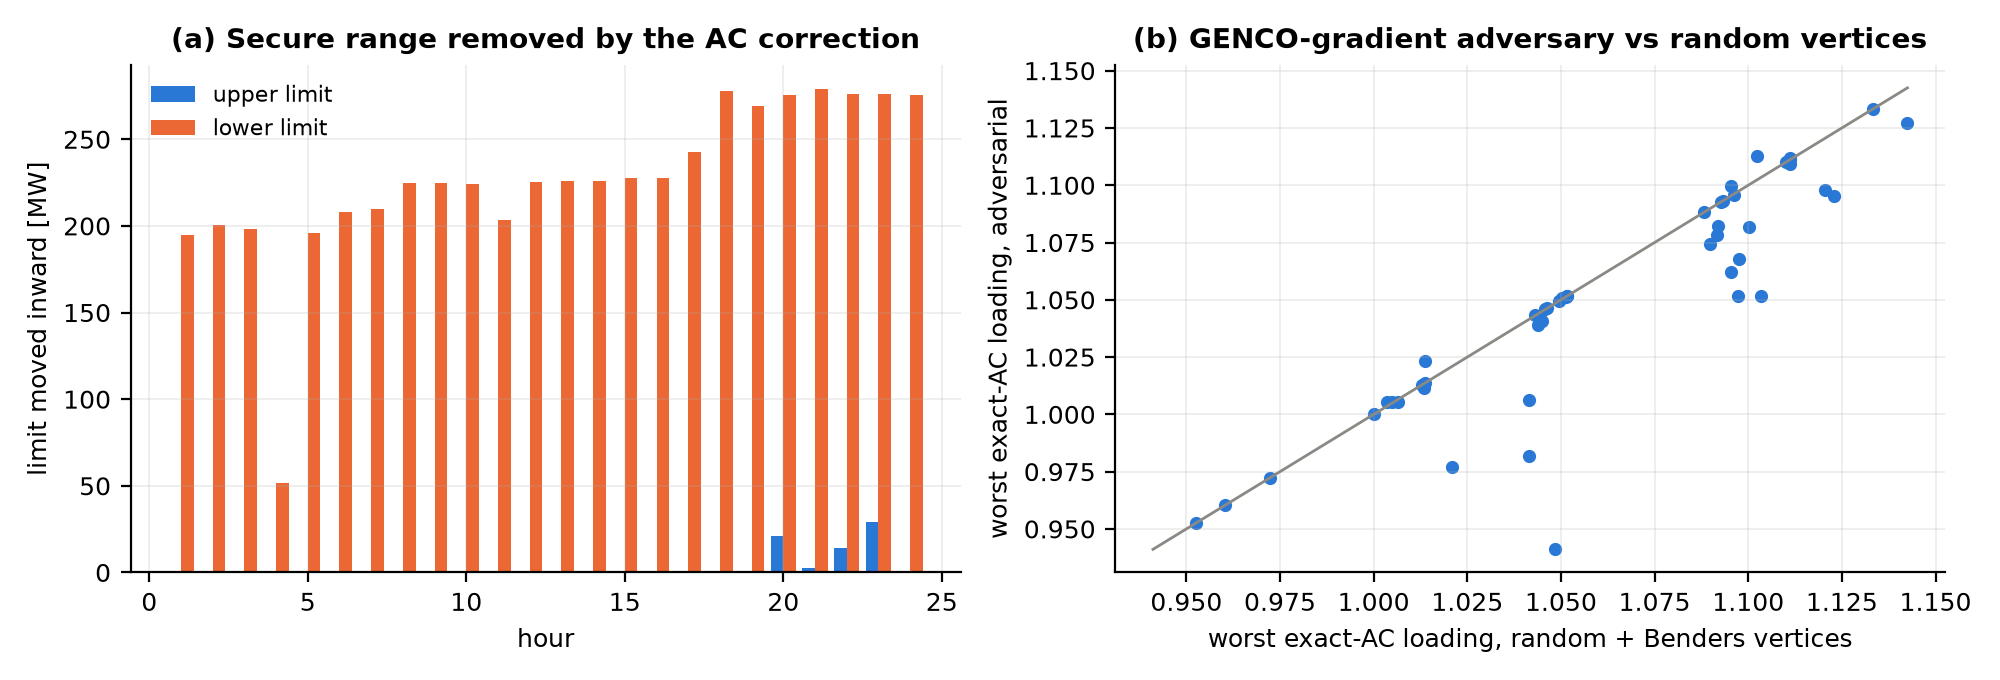
\includegraphics[width=0.78\textwidth]{../results/figures/fig4_ac_loop.png}
\caption{(a) Secure range removed by the AC correction, per hour and limit (MW the limit
moved inward). (b) Worst exact-AC loading at GENCO-adversarial vs.\ Benders/random
vertices (one point per search).}
\label{fig:ac}
\end{figure*}

\subsection{Extension: second-life EV batteries (E5)}
Placing second-life EV batteries ($P=\mathrm{SoH}\cdot0.35\cdot$ PV capacity, 20 sites,
3.6\,p.u.\ in total) as follower resources widens the certified DC range by
\NBessGainMeanMw\,MW on average (\NBessGainMinMw--\NBessGainMaxMw), i.e.\ \NBessFracMean\
of the theoretical $2P_\mathrm{bess}$. The worst-case points are AC-insecure in
\NBessAcInsecure\ of \NBessRows\ cases with batteries and \NNobessAcInsecure\ of 48
without, so the AC correction of E4 is needed with batteries too.
